\chapter[Experimental setup]{Experimental setup}

\section[Main beam accelerating structure]{The TD26 accelerating structure}

\section[Linac and dogleg]{The LINAC and the Dogleg}
fdsfgvd


\begin{landscape}
\begin{figure}
\centering 
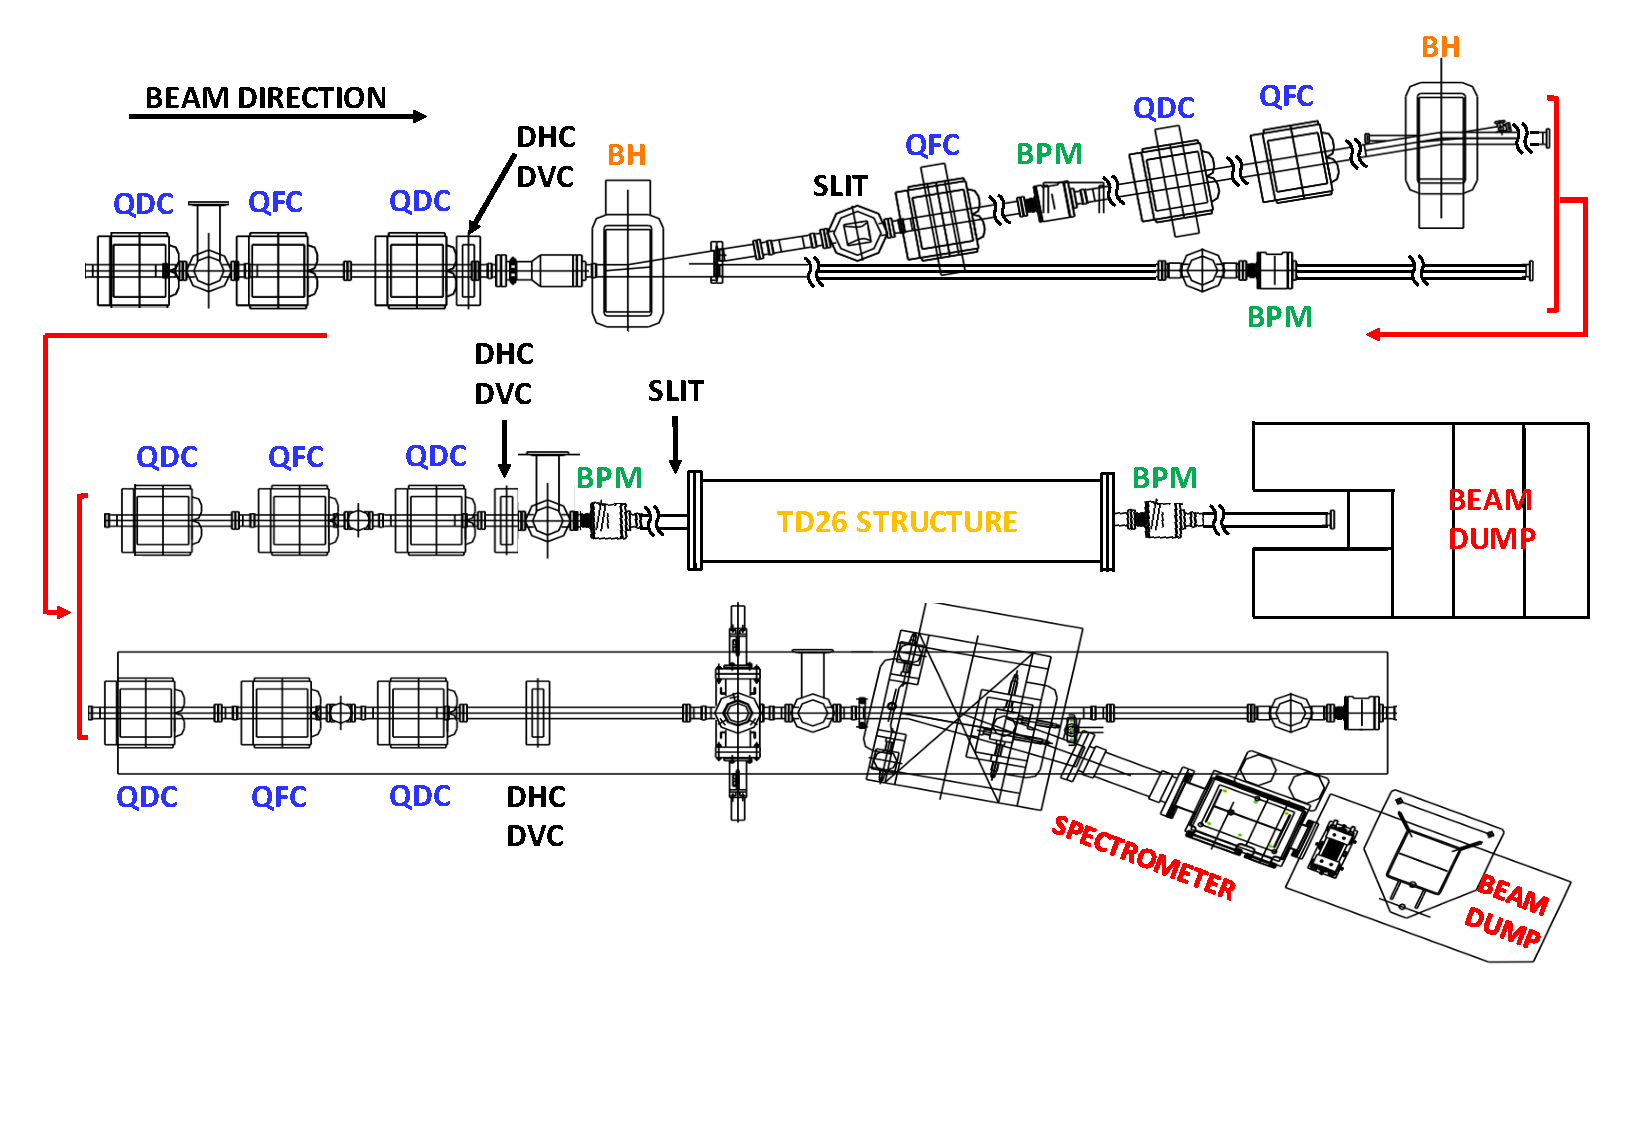
\includegraphics[scale=0.78]{pictures/modified_pets.pdf}
\caption{Simplified layout of optics and beam instrumentation of the dogleg line, adapted from technical drawings and facility layout \cite{EDMS:CTF3}. Legenda: QFC(QDC): focusing(defocusing) quadrupole; DHC(DVC): horizontal(vertical) dipole corrector; BH: bending magnet in horizontal plane; BPM: beam position monitor}
\label{dolaut}
\end{figure}
\end{landscape}


\section[RF power generation]{RF power generation}



\section[DAQ system]{DAQ system}

\subsection[Hardware]{Hardware}

\subsection[Online triggers]{Online triggers}

describe the online, but then the offline is in the next chapter

\section[Other systems]{Other systems}

mention here thermal systems for the structure and something else ???

